%%%%%%%%%%%%%%%%%%%%%%%%%%%%%%%%%%%%%%%%%%%%%%%%%%%%%%%%%%%%%%%%%%%%%%%%
\section{Products, primes and cuts}\label{sec:products}
%%%%%%%%%%%%%%%%%%%%%%%%%%%%%%%%%%%%%%%%%%%%%%%%%%%%%%%%%%%%%%%%%%%%%%%%

\subsection{Cuts}

\begin{definition}
A meander of order $N$ has a \emph{cut} at $m$, for $1\le m\le N-1$, if no lower arch passes over
gap $2m$, the crossings $2m$ and $2m+1$ are joined by a short upper arch, and exactly one other upper
arch passes over gap $2m$.
\end{definition}

Intuitively, a cut is a thin neck: the road passes from the left part of the river to the right part
exactly twice, once along the short arch and once along the arch over it. Figure~\ref{fig:cut} shows
an example. The product of Section~\ref{sec:growth} creates exactly such a neck.

\begin{theorem}[products and cuts]\label{thm:cuts}
The product $(G,H)\mapsto G\cdot H$ of Section~\ref{sec:growth} is a bijection from pairs of meanders
of orders $m$ and $N-m$ onto meanders of order $N$ with a cut at $m$. Moreover the cuts of $G\cdot H$
are the cuts of $G$, the position $m$, and the cuts of $H$ shifted by $m$.
\end{theorem}

\begin{proof}[Key idea]
The product creates the short arch $\{2m,2m+1\}$ and the arch $\{x,y\}$ over it, and no lower arch
passes over the gap, so it has a cut at $m$. Conversely, at a cut, replacing the two upper arches
over the gap, $\{x,y\}$ and $\{2m,2m+1\}$, by $\{x,2m\}$ and $\{2m+1,y\}$ separates the road into two loops, one on each
side, and these are the factors. A gap $2m'$ with $m'<m$ sees the same lower arches as in $G$ and the
same upper arches except that $\{x,2m\}$ became $\{x,y\}$, which passes over gap $2m'$ exactly when
$\{x,2m\}$ did; so cuts away from $m$ are those of the factors.
\end{proof}

So exactly $M_mM_{N-m}$ meanders of order $N$ have a cut at $m$, and for a uniformly random meander
\begin{equation}\label{eq:cutprob}
\Pr_N(\text{cut at }m)\;=\;\frac{M_mM_{N-m}}{M_N}\;=\;\frac{u_mu_{N-m}}{u_N}.
\end{equation}
In particular $\Pr_{2m}(\text{cut at }m)=e^{-D(m)}$: the doubling defect of Section~\ref{sec:growth}
is minus the logarithm of the probability of a cut at the middle.

\begin{figure}[t]
\centering
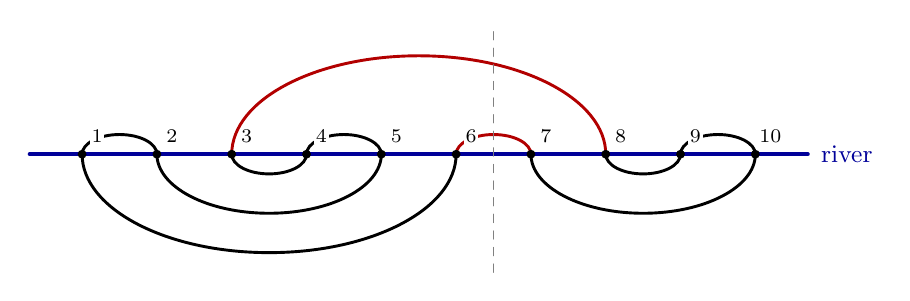
\begin{tikzpicture}[x=0.95cm,y=0.5cm,line cap=round]
  \draw[blue!60!black,line width=1.5pt] (0.3,0)--(10.7,0);
  \node[blue!60!black,anchor=west] at (10.75,0) {\small river};
  \begin{scope}[line width=1.05pt]
    \draw (1,0) arc[start angle=180,end angle=0,radius=0.5];
    \draw[red!70!black] (3,0) arc[start angle=180,end angle=0,radius=2.5];
    \draw (4,0) arc[start angle=180,end angle=0,radius=0.5];
    \draw[red!70!black] (6,0) arc[start angle=180,end angle=0,radius=0.5];
    \draw (9,0) arc[start angle=180,end angle=0,radius=0.5];
    \draw (1,0) arc[start angle=180,end angle=360,radius=2.5];
    \draw (2,0) arc[start angle=180,end angle=360,radius=1.5];
    \draw (3,0) arc[start angle=180,end angle=360,radius=0.5];
    \draw (7,0) arc[start angle=180,end angle=360,radius=1.5];
    \draw (8,0) arc[start angle=180,end angle=360,radius=0.5];
  \end{scope}
  \draw[gray,dashed] (6.5,-3)--(6.5,3.2);
  \foreach \k in {1,...,10} {\fill (\k,0) circle[radius=1.6pt]; \node[fill=white,inner sep=0.6pt,font=\scriptsize] at (\k+0.2,0.45) {\k};}
\end{tikzpicture}
\caption{A meander of order $5$ with a cut at $m=3$ (dashed line, gap $6$). No lower arch passes
over the gap; above it there is the short arch $6$--$7$ and one other arch, $3$--$8$ (both red).
Replacing these two arches by $3$--$6$ and $7$--$8$ splits the road into the running example of
Figure~\ref{fig:running} on crossings $1$--$6$ and a meander of order $2$ on crossings $7$--$10$.}
\label{fig:cut}
\end{figure}

\subsection{Prime meanders}

A meander is \emph{prime} if it has no cut. By Theorem~\ref{thm:cuts} and induction on the smallest
cut, every meander is a product $Q_1\cdot Q_2\cdots Q_k$ of primes in exactly one way, and the
product is associative. With $P_n$ the number of prime meanders of order $n$,
$\mathcal M(z)=\sum_{n\ge1}M_nz^n$ and $\mathcal P(z)=\sum_{n\ge1}P_nz^n$, this says
\[ 1+\mathcal M(z)\;=\;\frac1{1-\mathcal P(z)} . \]
The first values are $P_n=1,1,5,27,175,1255,9699,79253,676429,\ldots$, and $P_{32}/M_{32}=0.794$.
Write $U=\sum_n u_n=\mathcal M(1/\mu)$, which is finite by Theorem~\ref{thm:sumu} below. Then
$\mathcal P(1/\mu)=U/(1+U)\le1/5$. In the language of renewal theory, $(u_n)$ is a \emph{transient}
renewal sequence: a meander is a sequence of prime blocks, and the weights $P_n\mu^{-n}$ of the
possible blocks add up to less than one. That a positive fraction of meanders is prime is not
proved.

\subsection{The sum of \texorpdfstring{$u_n$}{u\_n}}

Let $X_N$ be the number of meanders of order $N$ with one marked exterior upper arch (one not
enclosed by another upper arch), so that $M_N\le X_N\le NM_N$. By reflection in the river, $X_N$ also counts meanders with a marked exterior
lower arch.

\begin{theorem}\label{thm:sumu}
$\sum_{n\ge1}u_n\le1/4$.
\end{theorem}

\begin{proof}
Two facts are needed. First, the gaps other than the two ends over which no lower arch passes are
exactly the gaps between consecutive exterior lower arches, so a meander with $\eta$ exterior lower arches has $\eta-1$ of them.
Second, the meanders of order $N$ in which no lower arch and exactly two upper arches pass over gap
$2m$ number exactly $X_mX_{N-m}$. Indeed, if the two upper arches are $\{p,r\}$ and $\{p',r'\}$ with
$p<p'\le2m<r'<r$, replacing them by $\{p,p'\}$ and $\{r',r\}$ gives a meander on each side, each with a
marked exterior arch, and this is reversible; the case $p'=2m$, $r'=2m+1$ is a cut.

Counting only the gaps over which no lower arch and exactly two upper arches pass, we get
\[ X_N-M_N\;=\;\sum_\Gamma(\eta(\Gamma)-1)\;\ge\;\sum_{m=1}^{N-1}X_mX_{N-m}, \]
where the sum is over meanders $\Gamma$ of order $N$ and $\eta(\Gamma)$ is the number of exterior lower
arches.
With $\mathcal X(z)=\sum_nX_nz^n$ this says that $\mathcal X-\mathcal X^2-\mathcal M$ has
nonnegative coefficients. For $0\le z<1/\mu$ all three series converge, and
$\mathcal M(z)\le\mathcal X(z)-\mathcal X(z)^2\le1/4$. Letting $z$ increase to $1/\mu$ gives
$\sum_nM_n\mu^{-n}\le1/4$ by monotone convergence.
\end{proof}

In particular $u_n\to0$, and for every $\xi\in(0,1]$ at most $N^\xi/4$ of the $n\le N$ have
$u_n>n^{-\xi}$. From the exact counts and $\mu\le12.2970$, $U\ge\sum_{n\le32}M_n\,12.297^{-n}>0.1032$, so
\[ 0.1032\;\le\;U\;\le\;0.25 . \]
A numerical estimate, which assumes the power law~\eqref{eq:law} for the tail, is $U\approx0.1037$.

\subsection{The number of cuts}

By~\eqref{eq:cutprob} the expected number of cuts of a random meander of order $N$ is
\[ \mathbb E_N[\#\text{cuts}]\;=\;\sum_{m=1}^{N-1}\frac{M_mM_{N-m}}{M_N}. \]
Every cut is a gap over which no lower arch passes, so the number of cuts is at most $\eta-1$, where $\eta$ is the number of exterior lower arches. The mean
number of exterior upper arches, which equals the mean number of exterior lower arches, is
$X_N/M_N$, and a short surgery at the marked exterior arch shows $2X_N\le M_{N+1}$~\cite{Repo}. Hence
\begin{equation}\label{eq:cutmean}
\mathbb E_N[\#\text{cuts}]\;\le\;\frac{M_{N+1}}{2M_N}-1\;\le\;\frac{R_\star}2-1 ,
\end{equation}
which is bounded by Theorem~\ref{thm:ratio}. The exact values are $0.338$, $0.270$ and $0.245$ at
$N=10$, $20$ and $32$, decreasing (Table~\ref{tab:cuts}).

\subsection{Cuts away from the ends}

\begin{proposition}\label{prop:cutbound}
There is a constant $C_{\mathrm c}$ such that for all $N\ge2$ and $1\le k\le N-1$, with
$s=\min(k,N-k)$,
\[ \Pr_N(\text{cut at }k)\;\le\;C_{\mathrm c}\,s^{-1/4}\sqrt{\log(s+1)} . \]
\end{proposition}

\begin{proof}[Key idea]
Write $\psi(k)=M_kM_{N-k}/M_N$, the probability of a cut at $k$; it is symmetric, so let $k\le N/2$.
Moving the cut by $t$ positions changes $\log\psi$ by a difference of two sums of $t$ terms
$\log(M_{i+1}/(\mu M_i))$, since the factors $\mu$ cancel. By Theorem~\ref{thm:rate} each term is at
most $\delta(i)=2C_{\mathrm r}\,i^{-1/4}\sqrt{\log(i+1)}$ in absolute value, with all indices at least
$k/2$. So for $t_0=\lfloor1/\delta(\lceil k/2\rceil)\rfloor$, about $k^{1/4}$, there are $t_0+1$
positions where the probability of a cut is at least $e^{-2}\psi(k)$. Their sum is at most
$\mathbb E_N[\#\text{cuts}]$, which is bounded by~\eqref{eq:cutmean}, so
$\psi(k)=O(\delta(\lceil k/2\rceil))$. Bounded $k$ are handled by enlarging the constant.
\end{proof}

Intuitively, the probability of a cut is nearly constant over stretches of about $s^{1/4}$
positions, and the total over all positions is bounded. So no neck far from both ends carries a positive fraction of meanders. Under the power law the true order is
$(N/(k(N-k)))^{\alpha}$, much smaller. The bound is not summable over positions, and a better ratio
rate would not make it summable, so it does not settle whether the cuts in the middle carry vanishing
total probability (Section~\ref{sec:subexp}).

\subsection{Near-cuts}\label{sec:nearcuts}

A cut is a very special neck. A meander of order $2m$ can also be nearly split at the middle in looser
ways. These looser events are the ones that remain visible when a large random meander is rescaled
to a continuum picture, as in Paper~D~\cite{PaperD}. Two results compare them with exact cuts.

\emph{Zero defect.} Say that a meander of order $2m$ is \emph{split at the middle} if its first $2m$
crossings form one stretch of consecutive crossings along the road. On a closed road, a set of
crossings is one stretch exactly when two road arches leave it, so this is the event that exactly two
arches pass over gap $2m$. Both arches are upper or both are lower, by parity, and the count in the
proof of Theorem~\ref{thm:sumu} gives $X_m^2$ for each case.

\begin{proposition}[zero defect]\label{prop:zerodefect}
$\Pr_{2m}(\text{split at the middle})=2X_m^2/M_{2m}$ exactly. Consequently, since
$M_m^2/M_{2m}=e^{-D(m)}$,
\[ 2e^{-D(m)}\;\le\;\Pr_{2m}(\text{split at the middle})\;\le\;\tfrac12R_\star^2\,e^{-D(m)} . \]
\end{proposition}

The inequalities follow from $M_m\le X_m\le M_{m+1}/2\le R_\star M_m/2$. So a split at the middle is a cut
at the middle up to a bounded factor: given a split, the probability of an exact cut is at least
$2/R_\star^2$.

\emph{Bounded defect.} More generally, say the first $2m$ crossings have \emph{defect at most $K$} if
they differ in at most $K$ crossings from some stretch of $2m$ consecutive crossings along the road.
Such a meander has a \emph{near-cut} at the middle.
Each changed crossing adds at most two road arches leaving the set, so at most $2+2K$ arches pass over
gap $2m$. The next result bounds such meanders by exact products.

\begin{proposition}[linear-record completion]\label{prop:linrec}
For all $m,n\ge1$ and even $w\ge2$, the number of meanders of order $m+n$ in which at most $w$ arches
pass over gap $2m$ is at most $(64R_\star^3)^w M_mM_n$.
\end{proposition}

\begin{proof}[Key idea]
Suppose exactly $w$ arches pass over the gap, $w_\uparrow$ upper and $w_\downarrow$ lower; smaller numbers are handled
in the same way. Cut at the gap. The left half has $2m$ crossings and $w$ loose ends. Append
$w$ new crossings on the right and join the loose ends to them in nested order; this closes the half
into a system of at most $w$ closed roads, each of which meets the new crossings. Then merge the roads
from left to right along the new crossings: at each of the $w-1$ steps, either the next new crossing
is already on the current road, or one of three local moves joins the two roads, adding at most two
crossings. The record of the whole merge is a word of length $w-1$ in four letters, one letter per
step. Because the steps follow a fixed left-to-right schedule, the word determines where each move
happened, so the half is recovered from the completed meander and the word. This gives at most $4^{w-1}R_\star^{3w/2}M_m$ left halves with given $w_\uparrow$ and $w_\downarrow$, the factor
$R_\star^{3w/2}$ paying for the at most $3w/2$ extra orders. The same holds on the right, and the two
halves are glued across the gap in only one way.
\end{proof}

\begin{corollary}\label{cor:defect}
For every $K\ge0$,
\[ e^{-D(m)}\;\le\;\Pr_{2m}(\text{defect at most }K)\;\le\;(64R_\star^3)^{2K+2}\,e^{-D(m)} . \]
\end{corollary}

So near-cuts with defect $K$ are at most a factor $e^{O(K+1)}$ more likely than exact cuts. For a
slowly growing defect, $K=o(\log m)$, the two probabilities agree up to a factor $m^{o(1)}$, so they
decay with the same power of $m$ if either decays like a power.
